\section{A New Model}

\subsection{Definitions}

To overcome the limitations of classical models, which focus on the 
equilibrium status that will take a long time to reach, this paper propose a
new model that enables effective simulation on early-stages of a system using 
rejuvenation.  The new model works as the follows. It is initialised to a 
working state and its {\it software rejuvenate schedule} is set to time $T$.  
The failure rate during the working period is a function of the elapsed working 
time $t$.  A failed system takes $t_f$ time to repair.  At the end of a repair 
process or after working for $T$ time, the system enters to the rejuvenation 
process for $t_r$ time before being set to the initial working state.  Figure 
\ref{model_new} gives the transition digram for the new Model, which consists 
of  the following 3 {\it categories} of states:

\begin{itemize}
 \item {\tt W($\tau$), $0 \leq \tau < T$} the state that the system has running 
without failure for $\tau$ time;
 \item {\tt R($\tau$), $0 \leq \tau < t_r$} the state that the system has 
entered 
the rejuvenation process for $\tau$ time.
 \item {\tt F($\tau$), $0 \leq \tau < t_f$} the state that the system has 
failed 
for $\tau$ time, during which period no rejuvenation process has been invoked, 
but other repair processes, such as data restore, maybe performed.
\end{itemize}

For the convince of later discussions, this paper index possible state $x_i$ as 
follows:

\begin{defn}
\[ x_i = \left\{ 
  \begin{array}{l l}
    W(i)    &   0 \leq i < T \\
    R(i-T) &   T \leq i < T+t_r \\ 
    F(i-T-t_r) &   T+t_r \leq i < T+t_r+t_f \\     
  \end{array} \right.\]
\end{defn}

Let $X_t$ be the state of the system at time $t \geq 0$, then the process $X = 
(X_t, t \geq 0)$ is a stochastic process.  If time is a discrete value in the 
model, the process has discrete time and discrete state space.  
If time is a  continuous value in the model, the process has 
continuous time and continuous state space.  




\begin{figure}
  \label{model_new}
  \centering       
  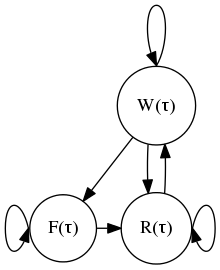
\includegraphics[scale=0.5]{model.png}
  \caption{New Model}
\end{figure}


\subsection{Cast Continues State Space to Discrete State Space}

As Section \ref{discrete_model} will show, a standard Markov Chain can be 
defined if time is treated as a discrete value.  Section 
\ref{discrete_simulation} will give the simulation process corresponding to 
the Markov Chain.  Although a general Markov process can be defined similarly 
for the case where time is a continuous value, unfortunately, the general 
Markov process does not have a precise simulation method.  Therefore, this 
paper converts the continuous case to an approximate discrete case, where a 
simulation method can be applied.  

To convert a model with continuous state space to one with discrete state space,
a new time unit, $\Delta t >  0$, is picked such that 
$T/\Delta t$, $t_r/\Delta t$, and $t_f/\Delta t$ are integers.  Let $pdf$ be 
the failure density function in the continues model, then the failure massive 
function at $T+\Delta t$ in the discrete model is 

\begin{equation}
pmf(T+\Delta t) =  \int_{T}^{T+\Delta t} pdf(t) dt
\end{equation}

Finally, times $t$ in the continuous model can be converted to $t/\Delta t$ in 
the new discrete model.

\begin{comment}
\subsubsection{The Transaction Probability Density}

Let $p_{ij}$ be the probability of moving from $X_i$ to $X_j$ and $0 \le j-i 
\le 
min\{T, t_r, t_f\}$.  
We have:

\begin{equation}
p_{ij} = 
\begin{cases} 
\frac{R(k+j-i)}{R(k)}    &  if\ x_i = W(k), \\ &\hspace{12pt}  x_j = W(k+j-i), 
\\ &\hspace{12pt}  0\leq k <T+i-j; \\

\frac{R(T)}{ R(k)}     &  if\ x_i = W(k),   x_j = F(l), \\ &\hspace{12pt}  
0\leq 
k < T, 0 \leq l < j-i; \\ 

\frac{R(T)}{R(k)}     &   if\ x_i = W(T-k),   x_j = R(k),\\ &\hspace{12pt}   0 
\leq k < j-i; \\

\int_{0}^{w} f(x)dx     &  if\ x_i = R(k),   x_j = F(l), \\ &\hspace{12pt}  
0\leq k < t_r, 0 \leq l < t_f; \\ &\hspace{12pt}  w = (j-i)-(t_r-k)-(t_f-l) \\

1     &  if\ x_i = R(k),  x_j = R(k+j-i),\\ &\hspace{12pt}   0\leq k <t_r+i-j, 
\\
       &  or\ x_i = F(k),   x_j = F(k+j-i),\\ &\hspace{12pt}   0\leq k 
<t_f+i-j, 
\\     
       &  or\ x_i = F(t_f-k),   x_j = R(k),\\ &\hspace{12pt}   0 \leq k < t_r, 
\\      
       &   or\ if\ x_i = R(t_r-k), \\ &\hspace{12pt}  x_j = W(k),   0 \leq k < 
T; \\       
0     &   otherwise
\end{cases}
\end{equation}
\hspace{90pt} where $0 \le j-i \le min{T, t_r, t_f}$
\end{comment}


\subsection{Discrete Model as a Markov Chain}
\label{discrete_model}

\subsubsection{Probability Mass Function and Failure Rate}

Let $f(t)$ be the probability mass function (pmf) which represents the 
probability that, without software rejuvenation, the system will fail when 
being running for exactly $t$.  We can derive its reliability function ($R(t)$) 
and the failure rate function ($\lambda(t)$) as follows:

\begin{subequations}
\begin{align}
R(t) & = 1- \sum \limits_{i=1}^{t-1} f(t) & t > 0 \label{discrete_reliability}\\
\lambda(t) & = f(t)/R(t)  & t>0 \label{discrete_failure_rate}
\end{align}
\end{subequations}

Intuitively, $R(t)$ is the probability that the system can survive for as least 
$t$ time and $\lambda(t)$ is the probability that the system, which has 
survived for time $t$, fails at the next moment.

\subsubsection{The Transaction Matrix}

We define the transaction matrix $P$ whose $(i,j)$th element is the probability 
of moving from $x_i$ to $x_j$ in exactly {\it one} unit of time,  we have:

\begin{equation*}
p_{ij} = 
\begin{cases} 
1 - \lambda(k) & if\ x_i = W(k), x_j = W(k+1),\\ &\hspace{12pt}  0\leq k <T-1; 
\\
\lambda(k)     & if\ x_i = W(k), x_j = F(0),\\ &\hspace{12pt}  0\leq k <T-1,  \\
1              & if\ x_i = W(T-1), x_j = R(0), \\
               & or\ x_i = R(k), x_j = R(k+1),\\ &\hspace{12pt}  0\leq k < 
t_r-1, \\
               & or\ x_i = R(t_r), x_j = W(0), \\
               & or\ x_i = F(k), x_j = F(k+1),\\ &\hspace{12pt}  0\leq k <t_f-1, 
\\
               & or\ x_i = F(t_f), x_j = R(0); \\
0              & otherwise
\end{cases}
\end{equation*}

It is easy to verify that $P$ satisfies the following two properties of {\it stochastic matrix}:
\begin{enumerate}[\itshape a\upshape)]
\item $p_{ij} \ge 0$, and
\item $\sum \limits_{i} p_{ij} = 1$.
\end{enumerate}



\subsubsection{Simulation}
\label{discrete_simulation}

Let $\mu_t$ be a row vector of probabilities so that $\mu_t(i)$ represents the 
probability that the system is at state $x_i$ at time $t$, we can inductively 
simulate $\mu_t$ as the follows:

\begin{subequations}
\label{discrete_simulation_mu}
\begin{align}
\mu_0 & =  \begin{cases}  \mu_0(0) = 1 & \\
    \mu_0(i) = 0 & 0 < i < T+t_r+t_f -1
\end{cases}  \label{mu_0}\\
\mu_t & = \mu_0 P  &  \label{mu_t}
\end{align}
\end{subequations}
Particularly, a row vector $\pi$ is called a stationary distribution if $\pi = 
\pi P$.

On the other hand, the Chapman-Kolmogorov Equation states the follows:

\begin{equation}
\label{discrete_CK}
p_{ij}(m+n) = \sum \limits_k p_{ik}(m)p_{kj}(n)
\end{equation}

where $p_{ij}(n)$ is the probability that the system moves from state $X_i$
to state $X_j$ with in exactly $n$ steps.  

A nice corollary of Equation \ref{discrete_CK} is:
\begin{equation}
\label{discrete_CK_corollary}
P_n = P^n
\end{equation}
where $P_n$ is the transaction matrix whose $(i,j)$th element is the probability 
of moving from $x_i$ to $x_j$ in exactly $n$ unit of time.

From either Equation \ref{discrete_simulation_mu} or Equation 
\ref{discrete_CK_corollary}, we have
\begin{equation}
\label{discrete_CK_corollary}
\mu_t = \mu_0 P^t
\end{equation}
a standard property of (time-homogeneous) Markov Chain.



\subsubsection{Utility Analysis}

Borrowed from economics, the notion of utility function is used to unifies
downtime cost analysis, availability analysis, and other variants in literature.

Let $u(i)$ be {\it utility function} that returns a real value if the system stays
at state $x_i$ for one unit of time, the $expected$ utility gained at time $t$,
and the $total$ utility gained until time $t$ are Equation \ref{discrete_utility_t}
and Equation \ref{discrete_utility_T} respectively.

\begin{subequations}
\label{discrete_utility}
\begin{align}
u_t  & =   \sum \limits_{i=0}^{T+t_r+t_f-1} u(i)\mu_t(i)  \label{discrete_utility_t}\\
U_t  & =  F_{i=0}^{t} u_i  \label{discrete_utility_T}
\end{align}
\end{subequations}
where $F$ is an accumulating function.


\newpage
CASE I: Availability Analysis

The utility function for availability analysis can be defined as:

\begin{equation}
\label{discrete_availability_utiliy}
u(i) =  \begin{cases}  1 & 0 \leq i < T \\
                       0 & T \leq i < T+t_r+t_f -1
\end{cases}
\end{equation}


The target of \citep{dohi2000statistical} is finding a value $T$ so that
$a = \sum \limits_{i=0}^{T+t_r+t_f-1} u(i)\pi(i) $ has a maximum value.
Notice that, the changes of systems availability before the Markov model 
reaches its steady-state $\pi$ is ignored in \citep{dohi2000statistical}.

For a safety crucial system expected to run $t$ time, users may want to use the 
following objective function instead.

\begin{equation}
\label{discrete_availability_minimum}
A_{min}(t) = \min_{i=0}^t u_i
\end{equation} 

The average availability of a system during its first $t$ time is:

\begin{equation}
\label{discrete_availability_average}
\bar{A}(t) = \frac{1}{ t }\sum \limits_{i=0}^{t} u_i
\end{equation}

If the system can reaches its steady-state $\pi$, one may expect that 
\begin{equation}
  \lim_{t\rightarrow \infty}{\bar{A}(t)} = a
\end{equation}

CASE II: Downtime Cost Analysis

As in \citep{huang1995software}, let $c_f$ and $c_r$ be the unit cost 
of the system in state $F$ and $R$ respectively, we have:

\begin{equation}
\label{discrete_downtime_utiliy}
u(i) =  \begin{cases}   0 & 0 \leq i < T \\
                       -c_r & T \leq i < T + t_r \\
                       -c_f & T + t_r \leq i < T + t_r + t_f
        \end{cases}
\end{equation}

The target of \citep{huang1995software} is finding a value $T$ so that
$c = \sum \limits_{i=0}^{T+t_r+t_f-1} u(i)\pi(i) $ has a maximum value.
Notice that, the changes of systems availability before the Markov model 
reaches its steady-state $\pi$ is ignored in \citep{dohi2000statistical}.
Actually, the expected total cost of running the system for $L$ time is:
\begin{equation}
\label{discrete_availability_total}
C(L) = \sum \limits_{t=0}^{L} u_t
\end{equation}

Only when the system can reaches its steady-state $\pi$, , one may expect 
that 
\begin{equation}
  \lim_{L\rightarrow \infty}{C(L)} = cL
\end{equation}

\newpage

CASE III: Benefit Analysis

The utility function in CASE I returns non-negative value while the utility 
function in CASE II returns non-positive value.  In reality, a software 
application gains revenue when it runs and cost resources to restart it when it 
is down.

Now consider an international Voice over Internet Protocol (VoIP) service 
provider, who implements a few independent front-end applications, each of 
which has the following utility function, where the unit of time is hour:

\begin{equation}
\label{discrete_benifit_utiliy}
u(i) =  \begin{cases}     r & 0 \leq i < T \\
                       -c_r & T \leq i < T + t_r \\
                       -c_f & T + t_r \leq i < T + t_r + t_f
        \end{cases}
\end{equation}

The goal is set a proper rejuvenation schedule $T$ to maximize the total 
utility gained during the expect service time $L$ defined as: 
\begin{equation}
\label{discrete_benifi_total}
U(L) = \sum \limits_{t=0}^{L} u_t = \sum \limits_{t=0}^{L}  \sum 
\limits_{i=0}^{T+t_r+t_f-1} u(i)\mu_t(i)
\end{equation}


\subsection{Reflection on Markov Processes}

The model in \citep{huang1995software} has its root in Continuous Time Markov 
Chain.  The model in \citep{dohi2000statistical} is a Continuous Time 
Semi-Markov Chain. Our model is a devised Discrete Time Markov Chain (DTMC) or 
a General Markov Process.

The General Markov Process is a precise model for software rejuvenation, but it 
may not have an analysitcal form for the simulation purpose.  Our devised 
DTMC adds a time parameter to standard DTMC, result in a special form of CTMC 
and SMC.

The problem of our devised DTMC is the expanded state space. Recall that the 
simulation process, $\mu_t = \mu_{t-1} P$, computes the product of a $1 \times 
n$ matrix and a $n \times n$ matrix, where $n$ is the number of states in the 
model.  It appears that the computational cost of the simulation 
process of the devised DTMC is impractical in a general case where $n$ is a 
large number.

Fortunately, the devised DTMC is an acceptable model for the software 
rejuvenation problem discussed in this paper for two reasons.  Firstly, 
non-zero values in the state transition matrix are sparsely distributed, and 
therefore matrix multiplication does not necessary require a long time to 
compute.   Secondly, similar to the process of reducing a continuous model to a 
discrete model, the state space of a descrete model can be further reduced for 
achieving better performance, with the cost of sacrifying accuracy.